\documentclass[a4paper,12pt]{article}
\usepackage{HomeWorkTemplate}

\usepackage[utf8]{inputenc}
\usepackage[]{babel}

\setlength{\parindent}{4em}
\setlength{\parskip}{0.5em}

\renewcommand{\baselinestretch}{1.5}


\usepackage{caption}
\usepackage{subcaption}
\usepackage{graphicx}
\usepackage{float}
\usepackage[utf8]{inputenc}
\usepackage{lmodern, textcomp}
\usepackage{circuitikz}
\usepackage[shortlabels]{enumitem}
\usepackage{hyperref}
\usepackage{tikz}
\usepackage{amsmath}
\usepackage{amssymb}
\usepackage{tcolorbox}
\usepackage{graphicx}
\usepackage{xepersian}
\settextfont{XB Niloofar}
\usetikzlibrary{arrows,automata}
\usetikzlibrary{circuits.logic.US}
\usepackage{changepage}
\newcounter{problemcounter}
\newcounter{subproblemcounter}
\setcounter{problemcounter}{1}
\setcounter{subproblemcounter}{1}
\newcommand{\problem}[1]
{
	\subsection*{
		پرسش
		\arabic{problemcounter} 
		\stepcounter{problemcounter}
		\setcounter{subproblemcounter}{1}
		#1
	}
}
\newcommand{\subproblem}{
	\textbf{\harfi{subproblemcounter})}\stepcounter{subproblemcounter}
}


\begin{document}
	\handout
	{اصول پردازش تصویر}
	{دکتر مصطفی کمالی تبریزی}
	{نیم‌سال اول 1399\lr{-}1400}
	{اطلاعیه}
	{سیدعلیرضا خادم}
	{97100398}
	{تمرین سری پنجم - سوال اول}
	زمان حدودی اجرا: 4 دقیقه و 30 ثانیه 
	
	ابعاد تصویر
	\lr{source}:
	$ 1200_{px} \times 630_{px} $
	
	ابعاد تصویر
	\lr{target}:
	$ 3973_{px} \times 2032_{px} $
	
	\section*{موارد لازم.}
	برای اجرا لازم است تا تصاویر 
	\lr{1.source.jpg}
	و
	\lr{1.target.jpg}
	در مسیر
	\lr{EX5\_Q1/}
	قرار داشته باشد. همچنین در پیاده‌سازی این سوال از کتابخانه‌های 
	\lr{cv2}
	،
	\lr{numpy}
	و
	\lr{scipy}
	استفاده شده است که قبل از اجرا بایستی این کتابخانه‌ها روی سیستم شما نصب باشد.
	\section*{روند کلی حل.}
	ایده کلی حل به این صورت است که مسئله را به حلِ معادله پوآسون دوبعدی با شرایط مرزی دیریکله تبدیل می‌کنیم. با توجه به این نکته که گرادیان در تصاویر اهمیت زیادی دارد و در واقع آنچه میتوان از تصاویر درک کرد تا حد زیادی به گرادیان تصویر وابسته است،  هدف ما این است که  گرادیانِ تصویر
	\lr{souce}ای 
	که میخواهیم در تصویر 
	\lr{target}
	قرار دهیم حفظ شود. استفاده‌ای که می‌خواهیم از گرادیان در حل این مسئله بکنیم به این صورت است که 
	\lr{blending}
	را به گونه‌ای انجام بدهیم گرادیان تصویر 
	\lr{source}
	بعد از قرار گرفتن در تصویر
	\lr{target}
	همچنان حفظ شود. برای انجام این کار لازم نیست که کاربر 
	\lr{object}
	مدنظر از تصویر
	\lr{source}
	را به صورت دقیق 
	\lr{segment}
	کند بلکه بهتر از که مقداری از 
	\lr{background}
	را هم داشته باشیم. (برای مثال کافیست که یک کانتور دورِ 
	\lr{object}
	کشیده شود.)
	 کاری که میخواهیم انجام بدهیم به این صورت است که این کانتور را از تصویر 
	\lr{source}
	برداریم و در تصویر
	\lr{target}
	قرار دهیم به طوری که گرادیان در ناحیه‌یِ داخل 
	\lr{contour}
	حفظ شود. خلاصه‌ای از روابطی که بایستی در این مسئله حل کنیم به صورت زیر است.
	
	\begin{figure}[H]
		\centering
		\begin{subfigure}{0.9\textwidth}
			\centering
			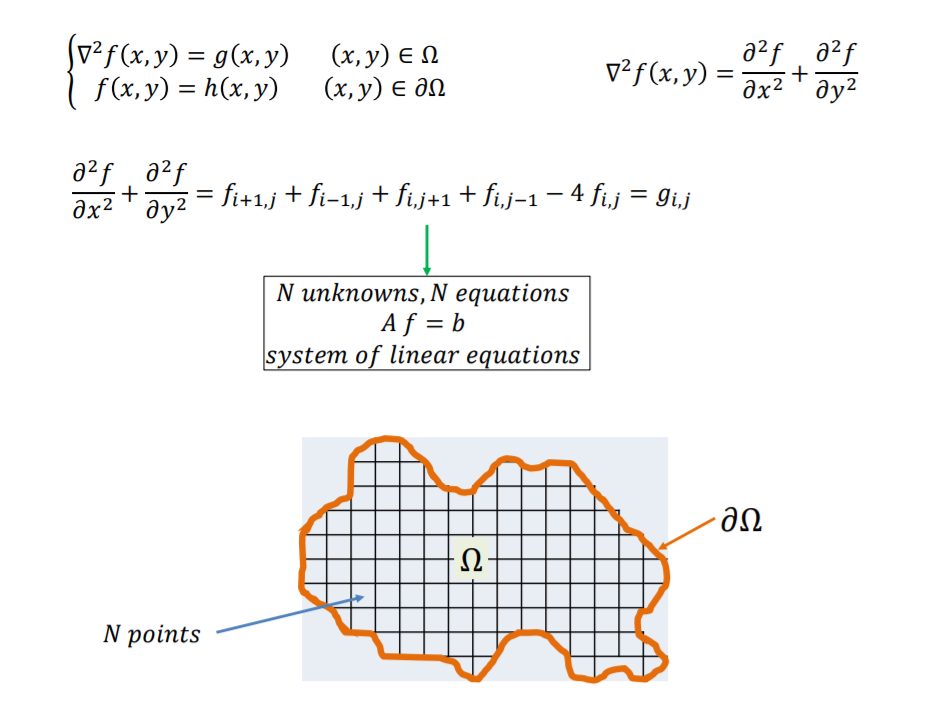
\includegraphics[width=\textwidth]{1.png}
		\end{subfigure}
	\end{figure}

همانطور که در روابط بالا نشان داده شده است از روشِ عددیِ
\lr{Finite Difference Method}
برای حل معادله پوآسون استفاده میکنیم. برای حل دستگاه معادله‌ای که در طی روند حل به آن برخواهیم خورد هم با توجه به این نکته که ماتریس ضرایب تعداد زیادی صفر دارد از کتابخانه 
\lr{scipy.sparse} 
برای حل این دستگاه استفاده می‌کنیم.

	
	\section*{توضیح کد.}
	برنامه در مجموع حاوی 2 فایل با فرمت
	\lr{.py}
	می‌باشد که توضیحات هر فایل در پایین آمده است.
	\subsection*{$\circ$ utilities.py}
	\subsubsection*{\lr{warp\_source\_image(source\_image, delta\_x, delta\_y, shape)}}
	این تابع تصویر 
	\lr{source}
	و مقدار جابه‌جایی در راستای
	\lr{x}
	و
	\lr{y}
	و ابعاد تصویر
	\lr{target}
	را به عنوان ورودی می‌گیرد و در خروجی تصویر با ابعاد 
	\lr{shape}
	برمی‌گرداند که در آن تصویر
	\lr{source}
	با یک
	\lr{translation}
	در مکان درست قرار گرفته است.
	\subsubsection*{\lr{blend(warped\_source, target, mask)}}
	این تابع تصویر وارپ‌شده‌ی 
	\lr{source}
	،
	تصویر 
	\lr{target}
	و 
	\lr{mask}
	را به عنوان ورودی می‌گیرد و بعد از اینکه ماتریس ضرایب 
	\lr{A}
	را با استفاده از تابع 
	 \lr{get\_mat\_A}
	 محاسبه کرد یک حلقه را اجرا می‌کند و برای هر 
	 \lr{channel}
	 ،
	 \lr{blending}
	 را انجام می‌دهد.
	 \subsubsection*{\lr{get\_mat\_A(mask, shape):}}
	 این تابع برای محاسبه‌ی ماتریس ضرایب استفاده می‌شود. 
	 \lr{mask}
	 و 
	 \lr{shape}
	 را به عنوان ورودی می‌گیرد. در ابتدا با استفاده از تابع 
	 \lr{get\_laplacian\_matrix}
	 ،
	 \lr{A}
	 را برابر با یک ماتریس پوآسون با ابعاد 
	  \lr{shape}
	  قرار می‌دهد و در ادامه درایه‌هایی از A که خارج از ناحیه سفید رنگِ
	  \lr{mask}
	  قرار دارد را برابر با همانی قرار می‌دهد. در نهایت هم با استفاده از تابع 
	  \lr{tocsc}
	  آن را به صورت 
	  \lr{csc}
	  در می‌آوریم تا با استفاده از کتابخانه 	  
	  \lr{scipy.sparse.linalg}
	  بتوان دستگاه معادله را حل کرد.	
	  \begin{figure}[H]
	  	\centering
	  	\begin{subfigure}{0.6\textwidth}
	  		\centering
	  		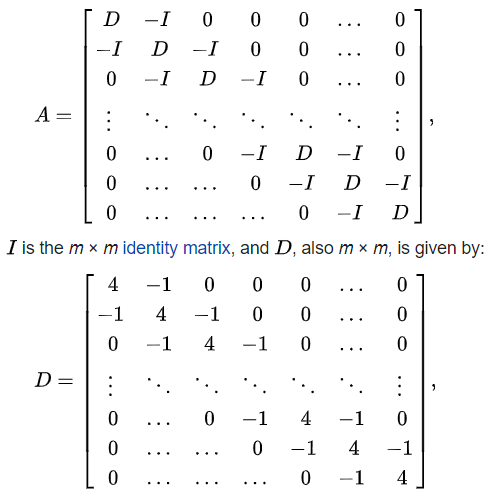
\includegraphics[width=.6\textwidth]{2.png}
	  	\end{subfigure}
	  \end{figure}
	  روابط دقیقتر را میتوان از این 
	  \href{https://en.wikipedia.org/wiki/Discrete_Poisson_equation}{لینک}
	  مشاهده کنید.
	 \subsubsection*{\lr{get\_mat\_b(A, source\_flat, target\_flat, mask\_flat)}}
	 این تابع ورودی‌هایی را که مشاهده می‌کنید را به عنوان ورودی می‌گیرد و 
	 \lr{b}
	 را ($ Af = b $) محاسبه می‌کند و به عنوان خروجی بر‌می‌گرداند.
	 \subsubsection*{\lr{scale(image, min, max)}}
	 این تابع یک تصویر را به عنوان ورودی می‌گیرد و مقدار 
	   \lr{intensity}
	   پیکسل‌هایی که 
	   \lr{intensity}
	   آنها کمتر از مقدار 
	    \lr{min}
	    است را برابر و مقدار 
	    \lr{intensity}
	    پیکسل‌هایی که 
	    \lr{intensity}
	    آنهابیشتر از
	    \lr{max}
	    است را برابر 
	    \lr{max}
	    قرار می‌دهد. در نهایت هم فرمت را به 
	     \lr{uint8}
	     تغییر داده و به عنوان خروجی برمی‌گرداند.
	\subsubsection*{\lr{blend\_channel(A, source, target, mask, channel, shape)}}
	این تابع ورودی‌هایی که مشاهده می‌کنید را به عنوان ورودی می‌گیرد و بعد از اینکه 
	\lr{source[:, :, channel]}،
	\lr{target[:, :, channel]} 
	و
	\lr{mask}
	را به صورت 
	\lr{flatten}
	در آورد، با استفاده از تابع 
	\lr{get\_mat\_b}
	مقدار 
	\lr{b}
	را محاسبه می‌کندو در ادامه با استفاده از تابع 
	\lr{spsolve}
	از کتابخانه 
	\lr{scipy.sparse.linalg}
	دستگاه معادله $ Af = b $ را حل می‌کند. در نهایت هم بعد از 
	\lr{reshape}
	کردن و 
	\lr{scale}
	کردنِ 
	\lr{f}
	،
	آن را به عنوان خروجی بر می‌گرداند.
	\subsection*{$\circ$ q1.py}
	در این فایل ابتدا تصاویر را لود می‌کنیم و در ادامه 
	\lr{result}
	را با استفاده از تابع 
	\lr{blend}
	محاسبه می‌کنیم و با نام 
	\lr{res1.jpg}
	در مسیر 
	\lr{EX5\_Q1/results}
	ذخیره می‌کنیم.
\end{document}
